%!TEX root = ../../../adrien_gomar_phd.tex

\subsection{Integrated results: similarity coefficients}
\label{sub:dream_ls_hb_sim_coeff}

Figure~\ref{fig:dream_ls_hb_unst_coeff} depicts the
unsteady variation of the thrust coefficient $C_T$ on 
both the front and the rear rotor. Actually, this is the
thrust coefficient associated to one blade multiplied by the
number of blade of the current rotor. This means that this
thrust coefficient does not represents the thrust generated
by the whole rotor. In fact, due to the phase-lag condition,
some blade unsteadinesses might cancel out each other.
Here, we want to assess the level of unsteadiness perceived by each blade
over one period.

The time is 
normalized by the reference period of the current rotor 
(the rotation frequency~$n$) and the thrust coefficient is normalized
by the temporal mean value. This allow to assess the unsteady variations
over one reference period. 


The level of unsteadiness is rather
the same on both rotors as it represents an envelope of almost
1\% of the temporal mean value. This level is not negligible and
justifies the use of unsteady methods on CROR configurations. 
Moreover, even though wakes are shed behind the front rotor
that impinge the rear rotor blades, the level of unsteadiness
perceived by the rear rotor is close to the front rotor ones.
\begin{figure}[htp]
  \centering
  \subfigure[]{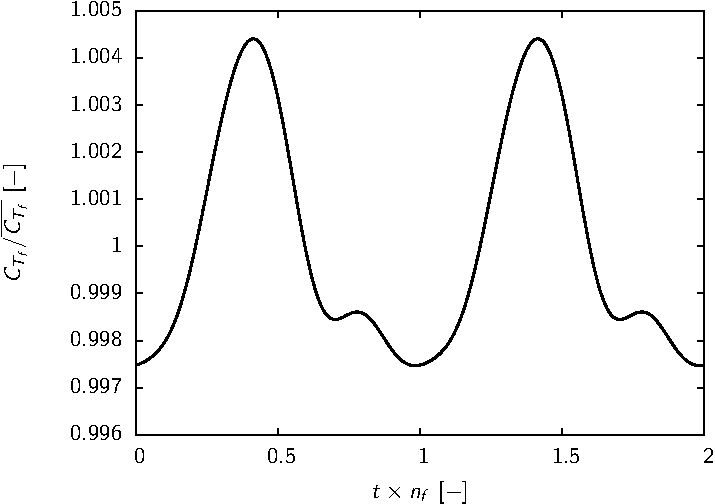
\includegraphics[width=.35\textwidth]{DREAM_LS_TSM_FORCES_INST_FRONT_PPT.pdf}}
  \subfigure[]{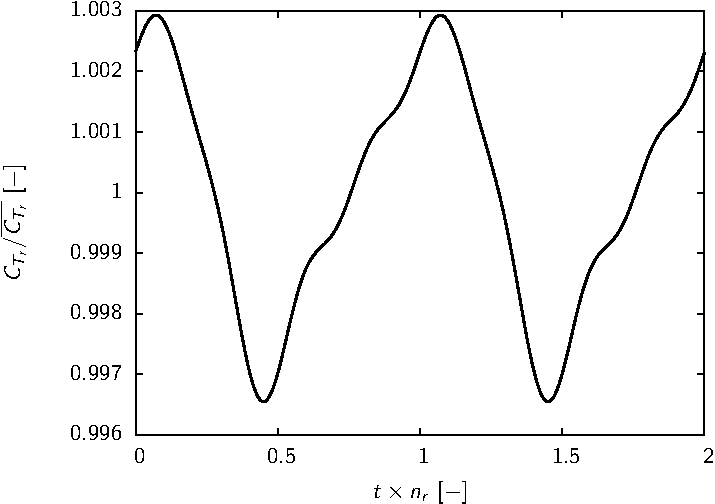
\includegraphics[width=.35\textwidth]{DREAM_LS_TSM_FORCES_INST_REAR_PPT.pdf}}
  \caption{Low-speed isolated configuration: unsteadiness seen by the rotors.}
  \label{fig:dream_ls_hb_unst_coeff}
\end{figure}

To assess in more detail the unsteady flow
field seen by the blade, an harmonic analysis on the
blades is performed in the following section.

\subsection{Two-dimensional results: harmonic blade response}
\label{sub:dream_ls_hb_blade_response}
